\documentclass[NET,a4,12pt,ngerman]{netforms}

\usepackage[utf8]{inputenc}
\usepackage{tumcommon/tumlang}
\usepackage{tumcommon/tumcontact}
% \usepackage{scrpage2}

% \documentclass[tikz]{standalone}

%
% This is a direct copy of the codes in section 2.9 of the package
% documentation (See page 45) https://mirrors.tuna.tsinghua.edu.cn/CTAN/graphics/pgf/contrib/pgfgantt/pgfgantt.pdf 
% except the color setting


\usepackage{pgfgantt}
\usepackage{xcolor}
\usepackage[utf8]{inputenc}
\usepackage{placeins}

\definecolor{barblue}{RGB}{153,204,254}
\definecolor{groupblue}{RGB}{51,102,254}
\definecolor{linkred}{RGB}{165,0,33} 


\geometry{%
	top=10mm,
	bottom=10mm,
	left=25mm,
	right=25mm,
	headsep=1.5cm,
	includehead,
}
% /////////////////////////////////////////////////
% \documentclass{article}
\usepackage{graphicx}
\graphicspath{ {./images/} }


% Alle Konfigurationsbefehle sind optional. Fehlende Befehle fueheren einfach
% zu "blank forms".

% Typ der Arbeit/Einstellung. Gueltige Argumente sind:
% bachelor,master,diplom,idp,gr,hiwi,other
% Falls 'other' gewaehlt wird, kann als optionales Argument eine spezielle Art
% von Abschlussarbeit angegeben werden, z.B. \type[Sklave]{other}. Andernfalls
% wird 'Other' als Standardbeschreibung gesetzt.
\type{bachelor}

% Informationen ueber den Studenten. Sollte selbsterklaerend sein.
\anrede{Herr}
\nachname{nachname}
\vorname{vorname}
\matrikel{matrikel}
\sunhalle{sunaccount}
\semester{1}{SoSe\,2016}
\studientelefon{}{tel}
\heimattelefon{}{--}
\studienadresse{strasse}{plz stadt}
\heimatadresse[adresszusatz=,appartment=]{}{}
\mail{student@tum.de}

% Informationen ueber die Arbeit. Sollte selbsterklaerend sein.
\themensteller{\NEThead}
\beginn{04}{2016}
\endt{08}{2016}
\betreuer{Stephan G\"unther, Maurice Leclaire}
\title{English Title of My Thesis}{Englischer Titel Meiner Arbeit}
\studiengang{Informatik}


% Falls \type{hiwi} gesetzt wurde, wird die Taetigkeit auf dem Aufnahmeformular
% des Lehrstuhls angegeben.
\taetigkeit{test}



% \pagestyle{scrheadings}
% \clearscrheadfoot
% \chead{\TUMheader{1cm}}

\renewcommand{\maketitle}{%
	\begin{center}
% 		\textbf{\introductoryheadline}%
        \textbf{Antrittsvortrag zur Masterarbeit}\\
		\Large%
		\textbf{Efficient and Accurate Hop-by-Hop Capacity Estimation}%
	\end{center}

	\footnotesize%
	\hrule
	\vskip1ex
	\begin{tabular}{ll}
		\thenamelabel: &  \textbf{Bakar Andguladze}\\
		\theadvisorlabel: & \text{Simon Bauer, Benedikt Jaeger}\\
		\thesupervisorlabel: & \chairhead\\
		\thebeginlabel: & {01/2021}\\
		\theendlabel: & {07/2021}\\
	\end{tabular}
	\vskip1ex
	\hrule
	\vskip4ex
}

\linespread{1.2}
\setlength{\parskip}{.5\baselineskip}

\begin{document}
\maketitle

\subsection*{Topic}

This Master's Thesis shall implement a capacity estimation method for Hop-by-Hop measurements.
The intended field of application is, for instance, enhancing the performance of network, traffic analysis, network monitoring, etc.  Our main motivation is to improve the ways of measuring the capacity of networks in the internet. As this would serve to enhance the quality of networks for which proper measurements of network capacity are required, in order to, for instance, diagnose potential problems in it.

There are quite a few measurement tools available, such as, PPrate\cite{PPrate}, Pathrate\cite{AbutOverview}, Pathchar\cite{AbutOverview}, etc. However the current State-of-the-Art methods have some significant flaws and limitations regarding our measurement goals, such as: 
\begin{itemize}
    \item Active tools require considerable amount of probes and this might cause network overload\cite{BrzozaThesis} which might, for example, result in lost packets and/or quyeue delays\cite{AbutOverview}.
    \item Passive tools analyze only ongoing traffic, therefore they're dependent on the traffic they observe. Also they require TCP servers to respond.
    Although they're widely used in practice and deliver reliable results, they're not sufficient to deliver all the desired information, such as the location of the narrow link.
\end{itemize}

Therefore our goal is to develop a new solution based on an active measurement technique that provides required features of both passive and active tools regarding our measurement objectives. We will try to implement the least possible intrusion without compromising accuracy. Also it will be able to find the first narrow link of the path by measuring the capacity of each hop in the network.
This new solution will be tested and evaluated by comparing it to the results of existing capacity measurement tools, i.e. PPrate implementation by Patryk Brzoza\cite{BrzozaThesis}, but in contrast to Brzoza's passive approach our tool will be based on an active measurement methodology. Moreover Brzoza's measurement tool was trying to find end-to-end capacity, while this thesis is concerned about measuring the capacity of each hop in the network and finding the narrow link. Hop-by-Hop measurements provide a better picture of a network and enables to take a closer look at potential issues.
This thesis is supposed to answer the following research questions:
\begin{itemize}
    \item How to measure network capacity hop-by-hop?
    \item How to optimize the trade-off between accuracy and intrusiveness regarding large-scale measurements?
    \item How robust is the proposed solution regarding the handling of cross-traffic, flow-interference and sudden path parameter changes?
    \item Are we able to locate the capacity bottlenecks of a network?
\end{itemize}



\subsection*{Approach}
This thesis includes three main parts: A, B and C:

Part A is the implementation of the tool. It will use active probing in order to generate TCP traffic to routers and gather the corresponding received ICMP messages. Afterwards a passive measurement method (based on PPrate\cite{PPrate}) will be applied to the gathered data. However, passive techniques are used for measuring end-to-end capacity. Therefore the main point of our approach is sending TCP packets with manipulated TTC values in a Traceroute-like manner.
For example, on Figure 1, we measure the capacity of C_1$ which is the narrow link of the path between the client C and the server S. Afterwards C_1$+C_2$ will be measured and checked if its capacity is smaller than the current narrow link. The measurement will continue to the following ones until it reaches the final endpoint.

\begin{figure}[h]
    \centering
    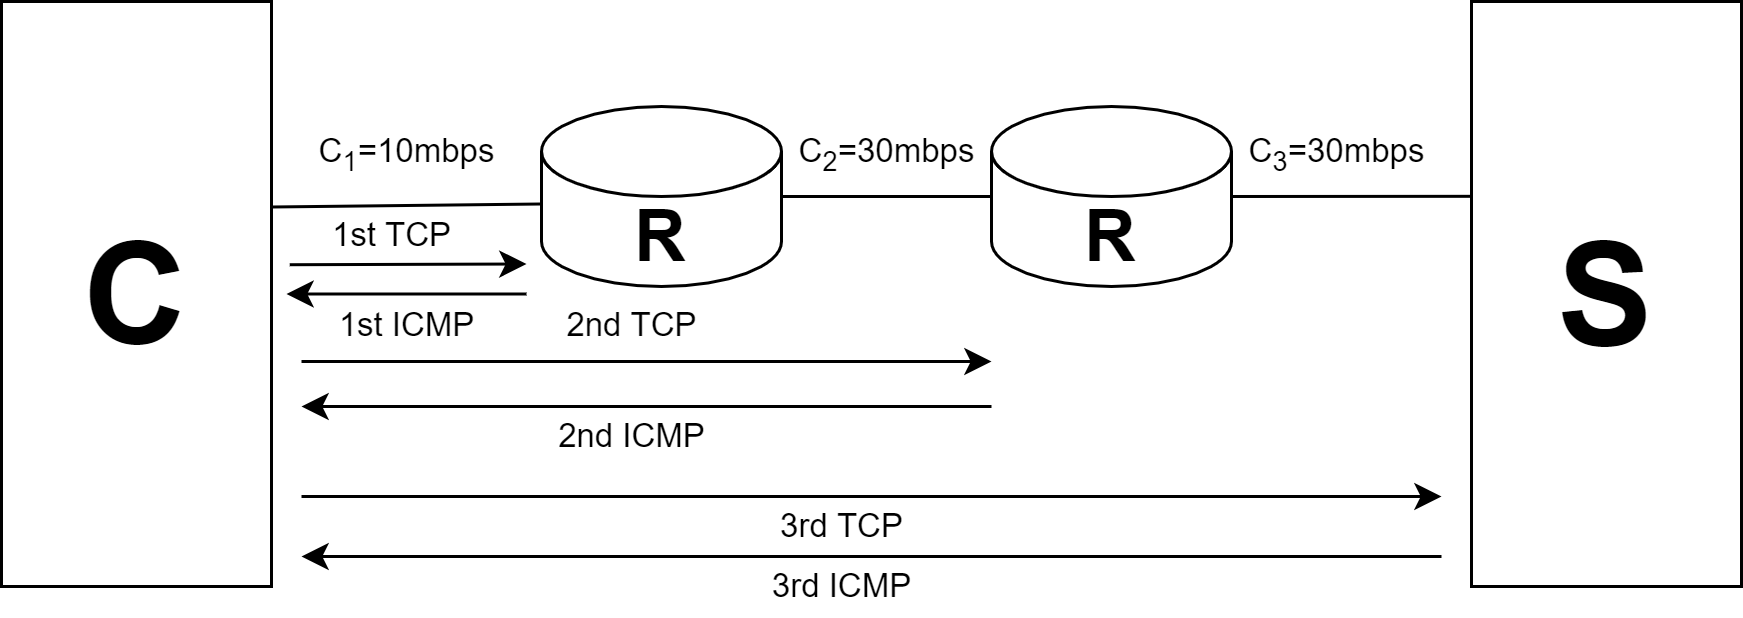
\includegraphics[scale=0.25]{images/NetworkDiag.png}
    \caption{Capacity measurement workflow  }
    \label{fig:mesh1}
\end{figure}


Part B is the evaluation. 
The first evaluation will be performed in a test environment using virtual network tool \textbf{\textit{mininet}}\cite{mininet}. For the maximum effectiveness various combinations of test parameters will be used, such as path lengths, cross traffic, capacities and delays.


We will compare the new solution with the existing TCP-based one, such as, Brzoza\cite{BrzozaThesis}. The different measurements will be conducted using the tools mentioned above and the results will be analyzed based on different test parameters and how these parameters influence the accuracy of measurements. 

Part C is the large-scale internet measurements conducted on the campus network. 
The second evaluation will be conducted on a real network by taking additional factors into consideration, such as size of traffic at different times and hours. 

The measurement tool will be developed in Python and C will be used for traffic generation. All the necessary operations will be performed on Ubuntu operating system.

The estimated timetable for this thesis can be seen below\colon

\begin{figure}[h]
    \centering
    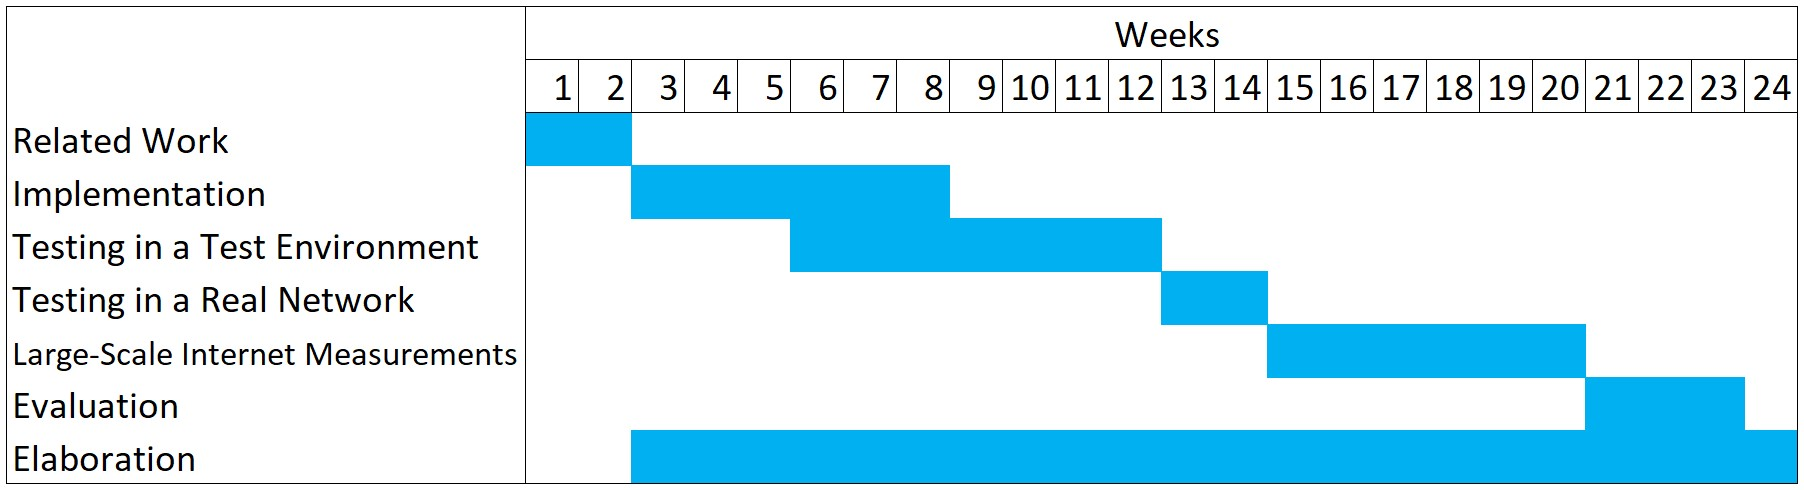
\includegraphics[scale=0.3]{images/GanttChart.jpg}
    \caption{Planned weekly schedule}
    \label{fig:mesh1}
\end{figure}



% \subsection*{Additional hardware requirements}
% \begin{itemize}
% 	\item 2 chassis for the USRPs \cite{chassiusrp}
% \end{itemize}

% \bibliographystyle{IEEEtran}
% \bibliography{IEEEabrv,lit}
% \clearpage
\FloatBarrier
\begin{thebibliography}{9}
\bibitem{PPrate} 
Taoufik En-Najjary, Guillaume Urvoy-Keller: PPrate: A Passive Capacity Estimation Tool. France, 2006

\bibitem{AbutOverview} 
Fatih Abut: Through the Diversity of Bandwidth-Related Metrics, Estimation Techniques and Tools An Overview. Adana, Turkey. 2018

\bibitem{BrzozaThesis} 
Patryk Brzoza: Implementation and Evaluation of Passive Capacity Estimation. 
Munich, 2018.

\bibitem{capest} 
Nicolas Kagami, et al.: CAPEST - Offloading Network Capacity and Available Bandwidth Estimation to Programmable Data Planes. Brazil, 2019

\bibitem{davrolis} 
Constantinos Dovrolis, et al. - Packet-Dispersion Techniques and a Capacity-Estimation Methodology. 2004

\bibitem{BrzozaGR}
Patryk Brzoza, et al.: Accuracy Optimization of Passive Capacity Estimation 

\bibitem{mininet}
R.L.S. De Oliveira, et.al. “Using Mininet for Emulation and Prototyping Software-Defined Networks" 2014


\end{thebibliography}

\end{document}
